\section*{Instrucciones:}

\begin{itemize}
    \item Entrega en un pdf las respuestas de los ejercicios que no requieran implementarse y añade una breve descripción de los programas que entregas (sus nombres y qué hacen).
    
    \item Los programas deben ir un zip. Debes realizar un programa en cada ejercicio que indique “Implemetar”.

    \item Recuerda que debes utilizar Java 21 LTS.

    \item \textbf{Si no compila utilizando Java 21LTS o si no se entrega la breve descripción de los
    programas se penalizará.}
\end{itemize}

\textbf{Tiempo de elaboración:} $\approx$ 2.5 hrs

\textbf{Total de puntos:} 100

\textbf{Nota:} En esta práctica \textbf{no} es necesario utilizar otros objetos de la biblioteca Concurrent de java que no hayan sido mencionados en el Contexto 1 de esta práctica, por ejemplo: \textit{getAndIncrement, ArrayBlockingQueue, ConcurrentLinkedQueue}. Muchos de estos objetos ya predefinidos en java son implementaciones linealizables: con consistencia, y en esta práctica no lo  necesitamos.

\section*{Ejercicios:}

\begin{enumerate}

\item El programa ColaSecuencial es una implementación de una cola secuencial. Implementa una Cola concurrente utilizando una pool de hilos (ExecutorService). No utilices candados ni synchronized.

\textbf{\textit{Ejercicio resuelto de forma practica y adjunto dentro del archivo comprimido}}

\hfill

\item Ejecuta varias veces tu implementación con diferentes secuencias de llamadas a métodos ¿Tu implementación funciona de acuerdo a lo que se espera de una cola o suceden inconsistencias? Por ejemplo,

1) Se hace enq(a), enq(b) y deq() y al final ambos elementos a y b están en la cola.

2) Se realiza un enq(a) y un enq(b) y la cola solo contiene al elemento a o b.

3) Se desencola dos veces el mismo elemento.

Si existe una ejecución así toma una captura pantalla del resultado de tu programa que lo ejemplifique.

\hfill

\textit{Hint: Para analizar si hay inconsistencias, utiliza la interfaz Future, solo ten cuidado con el método get() ya que fuerza a que el resultado del future sea devuelto en ese momento.}

\hfill

\textbf{Importante:} El orden en el que se suben las tareas con submit y se guardan en los futures, no es el orden en el que se realizan, solo es el orden en el que se les asignan a los hilos. Nuestro sistema es asíncrono, es decir, cada hilo puede tardarse más o menos en ejecutar la tarea que se le asignó.\\

\begin{itemize}
    \item Secuencia 1:

    Se hace enq(a), enq(b) y luego deq(), al final ambos elementos a y b deben estar en la cola.

    \begin{verbatim}
// secuencia 1
public static void main(String[] args) throws InterruptedException, 
 ExecutionException {
    int n_hilos = 4;
    ColaConcurrente2 queue = new ColaConcurrente2(n_hilos);
        
    ExecutorService executor = Executors.newFixedThreadPool(n_hilos);
        
    Future<?> future1 = executor.submit(() -> queue.enq("a"));
    future1.get();  // Esperamos a que termine de encolar "a"
        
    Future<?> future2 = executor.submit(() -> queue.enq("b"));
    future2.get();  // Esperamos a que termine de encolar "b"
        
    Future<?> future3 = executor.submit(() -> queue.deq());
    future3.get();  // Esperamos a que termine de desencolar "a"
        
    // Se imprime la cola para ver el estado después de las operaciones
    queue.print();  // Debe imprimir "b"

    executor.shutdown();  // Cierra el executor
    }
    \end{verbatim}

    El resultado esperado es:
    \begin{verbatim}
        Enqueued: a
        Enqueued: b
        Dequeued: a
        Printing queue
        b
    \end{verbatim}

    Y se obtuvo:
    \begin{verbatim}
    Enqueued: a
    Enqueued: b
    Dequeued: a
    Printing queue
    b
    \end{verbatim}  

    El resultado obtenido fue lo que esperábamos para la primera secuencia, esto indica que la implementación funciona correctamente para esta secuencia de operaciones:

    enq(a): Se encola correctamente el elemento a.

    enq(b): Se encola correctamente el elemento b.

    deq(): Se desencola correctamente el elemento a.

    print(): Se imprime correctamente el contenido de la cola, mostrando solo b.

    \item Secuencia 2: 

    enq(a): Se encola el elemento a.

    enq(b): Se encola el elemento b.

    deq(): Se desencola un elemento (debería desencolar a).

    deq(): Se desencola otro elemento (debería desencolar b).

    \begin{verbatim}
        // secuencia 2
    public static void main(String[] args) throws InterruptedException, 
    ExecutionException {
        int n_hilos = 4;
        ColaConcurrente2 queue = new ColaConcurrente2(n_hilos);

        Future<?> future1 = queue.enq("a");
        Future<?> future2 = queue.enq("b");
        future1.get(); // Espera a que se termine la primera tarea
        future2.get(); // Espera a que se termine la segunda tarea

        Future<?> future3 = queue.deq(); // Desencola el primer elemento
        future3.get();

        Future<?> future4 = queue.deq(); // Desencola el segundo elemento
        future4.get();

        // Imprime el estado final de la cola
        Future<?> future5 = queue.print();
        future5.get();
    }
    \end{verbatim}

    El resultado esperado es:
    \begin{verbatim}
    Enqueued: a
    Enqueued: b
    Dequeued: a
    Dequeued: b
    Printing queue
    \end{verbatim}

    Y el resultado obtenido fue:
    \begin{verbatim}
    Enqueued: b
    Enqueued: a
    Dequeued: b
    Dequeued: a
    Printing queue
    \end{verbatim}

    \begin{figure}[h]
    \centering
    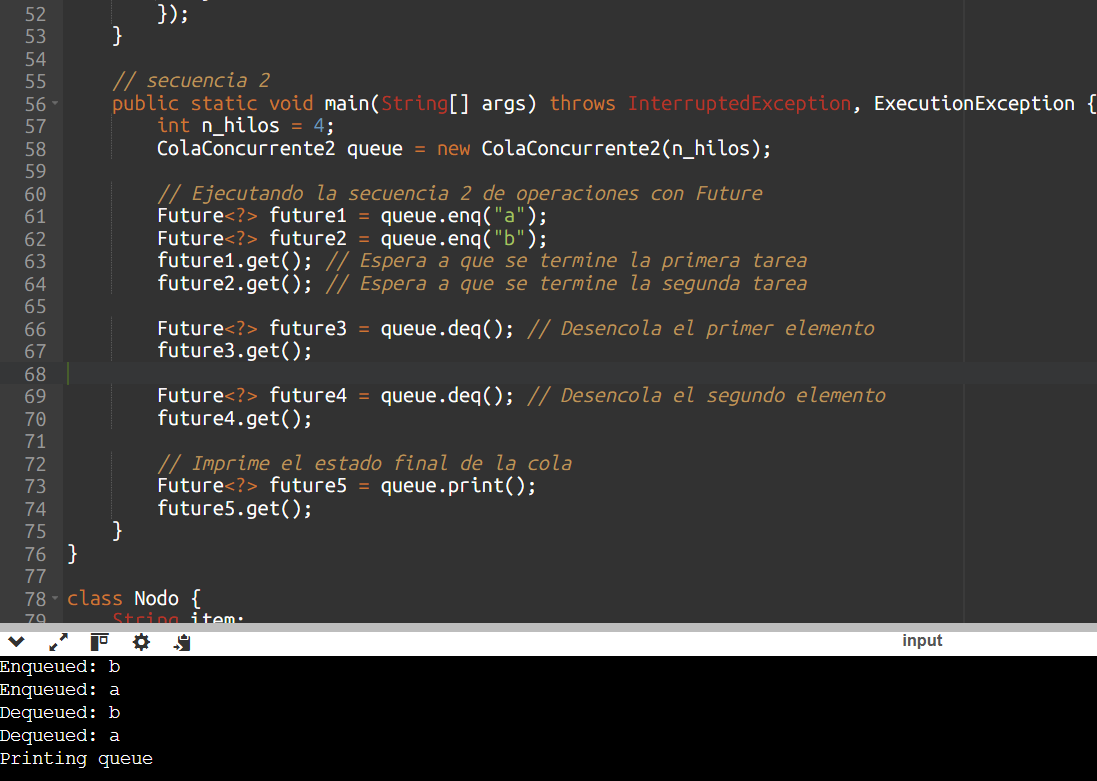
\includegraphics[width=8cm, height=7cm]{2 - sec 2.png}
\end{figure}

    El resultado obtenido muestra que las operaciones se ejecutaron en el orden contrario al esperado. 
    
    Es decir, se encolaron primero b y luego a.

    Se desencolaron b y luego a, en lugar de a y luego b.

    Esto es debido a que las tareas están siendo ejecutadas de manera asincrónica por los hilos del ExecutorService, y el orden de ejecución de las tareas no está garantizado, aunque las enviamos en un orden específico con submit.

    El problema es que las tareas de encolado (enq(a) y enq(b)) son asignadas a los hilos en el orden en que se ejecutan, pero eso no garantiza que se completen en el mismo orden. Como los hilos pueden ejecutarse de manera no secuencial, el resultado puede variar.

    Entonces, enq(a) puede ser ejecutada después de enq(b), esto provoca que b se encole primero y luego a. Para el desencolado, los hilos pueden procesar las tareas de desencolado en cualquier orden

    \item Secuencia 3:

    operaciones en la cola:

    enq(a)

    enq(b)

    deq() (Esto debe desencolar el primer elemento, que es a)

    deq() (Esto debe desencolar el siguiente elemento, que es b)

    deq() (Esta operación debería indicar que la cola está vacía)

    \begin{verbatim}
    // Secuencia 3
public static void main(String[] args) {
    int n_hilos = 4;
    ColaConcurrente2 queue = new ColaConcurrente2(n_hilos);
    try {
         Future<?> f1 = Executors.newSingleThreadExecutor().submit(() -> 
         queue.enq("a"));
         Future<?> f2 = Executors.newSingleThreadExecutor().submit(() -> 
         queue.enq("b"));
         f1.get(); // Espera a que termine la tarea de encolar "a"
         f2.get(); // Espera a que termine la tarea de encolar "b"
            
         Future<?> f3 = Executors.newSingleThreadExecutor().submit(() -> 
         queue.deq());
            f3.get(); // Espera a que termine la tarea de desencolar el primer 
            elemento

            Future<?> f4 = Executors.newSingleThreadExecutor().submit(() -> 
            queue.deq());
            f4.get(); 
            // Espera a que termine la tarea de desencolar el siguiente elemento

            Future<?> f5 = Executors.newSingleThreadExecutor().submit(() -> 
            queue.deq());
            f5.get(); 
            // Espera a que termine la tarea de desencolar el último elemento

            queue.print(); // Imprime la cola al final
        } catch (InterruptedException | ExecutionException e) {
            e.printStackTrace();
        }
    }
    \end{verbatim}

    El resultado esperado es:
    \begin{verbatim}
    Enqueued: a
    Enqueued: b
    Dequeued: a
    Dequeued: b
    Queue is empty
    Printing queue
    \end{verbatim}

    Y el resultado obtenido fue:
    \begin{verbatim}
    Enqueued: b
    Dequeued: tnull
    Printing queue
    Dequeued: a
    Dequeued: b
    Enqueued: a
    a
    \end{verbatim}

    \begin{figure}[h]
    \centering
    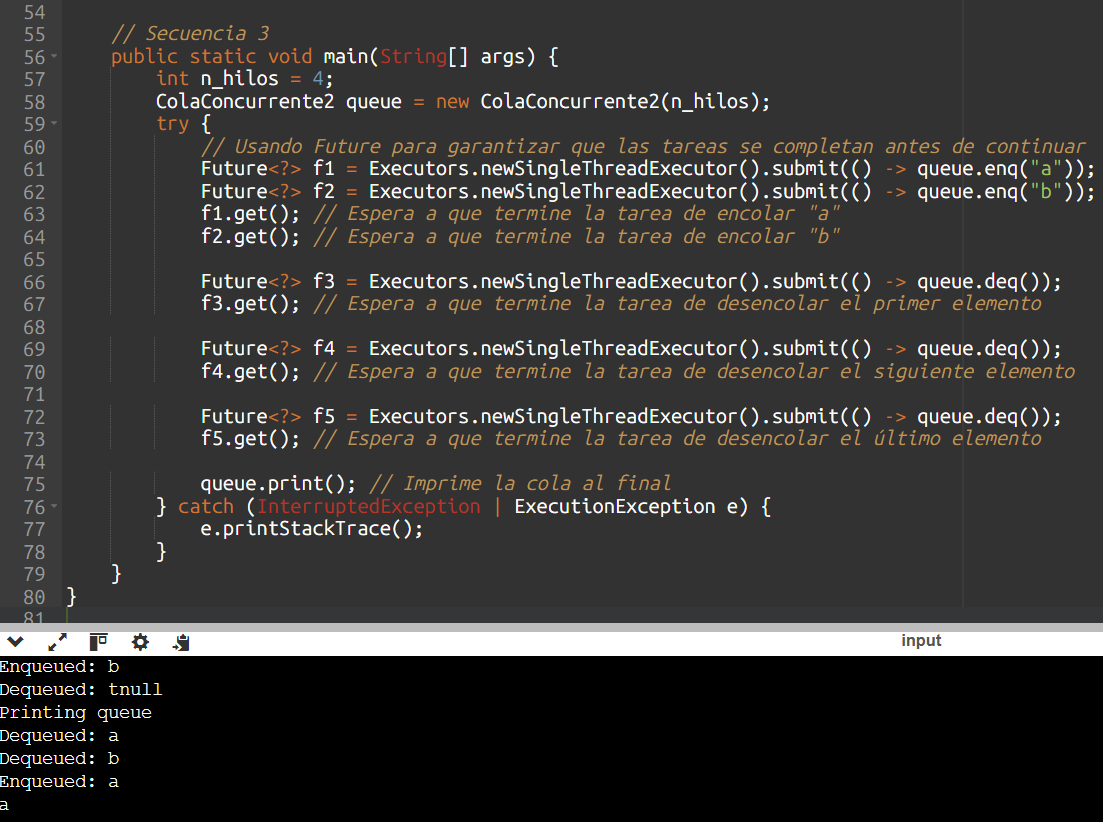
\includegraphics[width=8cm, height=7cm]{2 - sec 3.png}
\end{figure}
    Dequeued: tnull nos indica que la cola está manejando incorrectamente el nodo tnull (el nodo final), esto podría ser un problema en la lógica que maneja los nodos en la cola.

    Además, debería seguir el orden esperado de FIFO, pero parece que la secuencia se rompe.

    El nodo de tnull no debería estar involucrado en las operaciones normales de cola.
\end{itemize}

\hfill

\item ¿Existen data races o race-conditions? Explica en qué variables y porqué suceden.

Recordando ambas definiciones, mientras que una \textit{race-condition} ocurre cuando en una ejecución dos o más hilos acceden a un recurso compartido, una \textit{data race} es cuando dos o más hilos compiten por escribir al mismo recurso o lo llaman al mismo tiempo y po lo menos una es de escritura.

Observemos que nuestra implementación de nuestra cola secuencial, incluye el empleo de la clase \textbf{Lock}, misma que nos ayuda a tener un control flexible de nuestra zona crítica al momento de meter y o sacar elementos a la cola, pero esto a su vez impide que caigamos en problemas del tipo data races o race-conditions.

$\therefore$ No hay data races o race-conditions en nuestra implementación de cola concurrente.

\hfill

\item  Utiliza candados y/o synchronized en tu implementación de forma que los métodos enq() y deq() sean una sola sección crítica y contesta: ¿existen inconsistencias?
Importante: El orden en el que se suben las tareas con submit y se guardan en los futures, no es el orden en el que se realizan, solo es el orden en el que se les asignan a los hilos. Nuestro sistema es asíncrono, es decir, cada hilo puede tardarse más o menos en ejecutar la tarea que se le asignó.

\begin{figure}[h]
    \centering
    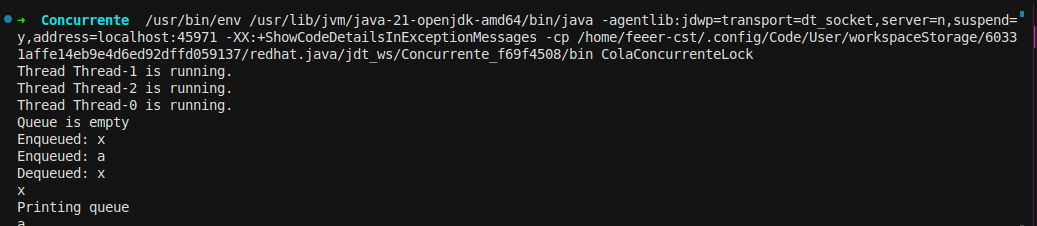
\includegraphics[width=0.8\textwidth]{images/Ejercicio4.png}
\end{figure}

Podemos ver que no hay inconsistencias, ya que hay locks en la sección crítica donde esto puedo fallar, en especifico el uso de lock()  y unlock() aseguran que un hilo a la vez pueda modificar la cola.
\hfill

\hfill

\item En una pool de hilos (ExecutorService), ¿si utilizamos más hilos equivale a un mayor throughput?

Argumenta porqué.

\hfill

\item \textbf{Problema.} Supón que perteneces a un equipo de trabajo en el cual estás a cargo de dar acceso a un servidor. Seis personas te pueden mandar tareas para que las ejecutes en el servidor. Las tareas del hilo 0 y 2 tardan 500ns, las del hilo 1 tardan 2000ns y las de los hilos 3, 4 y 5 tardan 3000ns.

Tienes la instrucción de no dar acceso a más de tres al mismo tiempo y de no aceptar al mismo tiempo las tareas del hilo 0 y 2. Diseña e implementa una solución. 

\textit{Hint:} Apóyate del programa Scheduler y Tarea, el semáforo inicializado en 3 representa que solo pueden entrar 3 al mismo tiempo, decide como utilizarlo en el programa Tarea (colocando sus métodos adquire y release); además, decide como utilizar un candado, para restringir aceptar las tareas de los hilos 0 y 2 al mismo tiempo.

\begin{itemize}
    \item ¿Tu implementación cumple con Justicia?

    A grandes rasgos, podemos tomar a la definición de Justicia como el hecho de que se respeten los tiempos de que hilo pidió el acceso a la sección crítica primero, es decir, que se cumpla FIFO (First In, First Out), analizando nuestro programa tras varias ejecuciones, podemos concluir que no en todos los escenarios se cumple esta propiedad.
    
    Un contraejemplo se da en los casos de las tareas 0 y 2 salgan una muy cerca de la otra (ej. 0,1,2,3,4,5), ya que las primeras 3 tareas que se procesarían serian 0, 1 y 3. 

    Otro de los problemas que se llega a presentar es que al haber tareas más rápidas que otras, se dan casos donde estas terminan ''salen'' antes que alguna predecesora.

    \item Sino es así, describe cómo podrías garantizarla.

    Entre la propuestas que podemos dar para solucionar este tipo de contratiempos, se puede implementar un manejo mas fino de esta excepción (que trabajen el 0 y el 2 a la vez), el controlar que a pesar de que haya tareas más rápidas que otras, de dar cierto margen para que acaben en el mismo orden que se iniciaron, e incluso podemos llevar esta análisis más profundo a cuestiones de la propia máquina virtual de Java donde por cuestiones de interpretación de la misma no es posible al 100\% (ej. en la imagen siguiente).

    \begin{center}
            \includegraphics[width = 8 cm]{images/Ejercicio6.png}
    \end{center}

    Veamos como la propia JVM, cambia el orden de los hilos de 0,3,5 a 0,5,3, que aunque parece insignificante, cuando manejamos grandes volúmenes de tareas tiene grandes repercusiones.
  
\end{itemize}
    
\end{enumerate}
